\chapter{Použité technologie}
\label{2-technologie}

\section{Django}

\begin{figure}[H] \centering
    
\includegraphics[width=160pt]{./pictures/django-logo.png}
    \caption[Django Logo]{Django Logo \cite{}}
	\label{fig:Django Logo}                                
\end{figure}

Django je open source prostředí, pro tvorbu webových aplikací. Django
je napsané v programovacím jazyku Python a pracuje na bázi
model-template-view. Model v tomto případě reprezentuje část, která je
schopna komunikovat a pracovat s databází. Templates určují obsah
zobrazení a jsou realizovány pomocí HTML. View zobrazuje daný obsah
koncovým uživatelům.

Django bylo vytvořeno v roce 2005 americkou společností The World
Company. Jeho první verze byla označena 0.90 a vyšla 16. listopadu
2005. Vývojáři pokračovali v jeho zdokonalování, kdy bylo během
následujících pár let provedeno několik aktualizací. V roce 2008 byla
vydána verze 1.0. Vývoj se nezastavil a po několika updatech byl v
roce 2013 vydána verze 1.5, která zajišťovala také podporu pro
Python 3, dříve pouze Python 2. Další velkou aktualizací bylo vydání nové
verze Django 2.0 na konci roku 2017. Ta zajišťovala plnou podporu pro
Python 3 a nadála už není možné pracovat s verzí Python 2. Aktuální
verze Djanga je 3.1, s tím že se plánuje v blízké době vydat verzi 3.2
po které by měl následovat další velká aktualizace v podobě Djanga 4.0,
která je plánována na začátek roku 2022. \cite{django}

\newpage


\subsection{Django - instalace a inicializace projektu}

Django je framework pracující v jazyce Python, pro jehož aktuální
verzi 3.1 je potřeba mít nainstalován verzi Python 3.6 nebo
vyšší. Nejjednodušší je pomocí příkazové řádky spustit příkaz {\tt pip
install django}, čímž by se měla nainstalovat nejaktuálnější verze
Djanga. Po instalaci lze pro zobrazení aktuální verze použít příkaz
django-admin --version. Po instalaci se opět pomocí příkazové řádky
provede vytvoření projektu v aktuální složce příkazem {\tt django-admin
startproject [název projektu]}. \cite{django-init} Tímto se vytvoří nový adresář který
vypadá následovně:

\begin{itemize}
	\item \lbrack Název projektu\rbrack /
	\begin{itemize}
		\item manage.py
		\item \lbrack Název projektu\rbrack /
		\begin{itemize}
			\item \_\_init\_\_.py
			\item setting.py
			\item urls.py
			\item asgi.py
			\item wsgi.py
		\end{itemize}
	\end{itemize}
\end{itemize}

\vspace{6px}

\textbf{\_\_init\_\_.py} určuje, aby s adresářem bylo zacházeno jako s celkem.
\vspace{6px}

\textbf{setting.py} zde se definují všechna nastavení Django projektu. 
\vspace{6px}

\textbf{urls.py} v projektovém adresáři definuje seznam URL adres na
úrovní projektu. Při založení je zde obsažena administrátorská
stránka.  \vspace{6px}

\textbf{wsgi.py} (Web Server Gateway Interface) slouží pro propojení
webového serveru s frameworkem Django, popřípadě jinými webovými
aplikacemi.  \vspace{6px}

\textbf{asgi.py} (Asynchronous Server Gateway Interface) byl do Djanga
přidán ve verzi 3.0 a je nástupce staršího WSGI. Výhodou WSGI oproti
ASGI je, že dokáže pracovat se složitějšími protokoly jako jsou
WsbSocket, IoT protokoly, HTTP2 a další. Umožňuje komunikovat přes
více linek a tedy posílat a přijímat více dat najednou.  \vspace{6px}

\textbf{manage.py} je automaticky vygenerován v novém adresáři a je
přítomen v každém Django projektu. Je to nástroj pro spouštění
specifických příkazů například pro spuštění aplikace nebo vytvoření
aplikací.

\newpage

Pomocí nástroje manage.py se v Djangu spouští řada důležitých
příkazů. Zde je výčet těch nejdůležitějších a jejich popis. \cite{django-admin-manage}

\begin{itemize}
\item {\tt python manage.py runserver} - tento příkaz spouští
  aplikaci na lokálním serveru. Standardně je to na adrese
  127.0.0.1:8000. Aplikace je po spuštění přístupná pouze z daného
  zařízení a není možné se k ní připojit ani v rámci lokální
  sítě. Pokud je při spuštěném serveru provedena nějaká změna v kódu,
  framework projde celý projekt pro nalezení případné chyby a změna se
  automaticky zobrazí ve výstupu.
	
\item {\tt python manage.py makemigrations [název aplikace]} -
  tento příkaz provede porovnání modelu a s databází. Pokud jsou
  nalezeny změny, vytvoří se nový soubor se stávajícími migracemi. Ten
  obsahuje SQL příkazy, jak by se měla vytvořit databáze podle modelu
  definovaném v aplikaci. Příkaz se definuje zadáním jména aplikace,
  potažmo aplikací, lze tedy vytvořit migrace pouze pro jednu nebo
  více aplikací, zadáním jejich názvů.

\item {\tt python manage.py migrate} - spuštěním tohoto příkazu se
  synchronizuje databáze s modelem podle migračního souboru, který je
  generovaný z příkazu \newline {\tt makemigrations}.
	
\item {\tt python manage.py inspectdb} - příkaz vytvoří schéma
  připojené databáze a uloží ho do paměti. Vytvoření model.py souboru
  se pak provede spuštěním příkazu {\tt python manage.py inspectdb
    > models.py}.

\end{itemize}

\newpage

\subsection{Django - tvorba aplikace}

Po založení projektu je potřeba vytvořit aplikaci. Počet použitých
aplikací v projektu není omezen a jejích výhodou je, že je lze
opětovně použít v dalších projektech. Aplikace se vytvoří příkazem{\tt
python manage.py startapp [nazev aplikace]}. \cite{django-init} Schéma je následující:

\begin{itemize}
	\item \lbrack Název aplikace\rbrack /
 	\begin{itemize}
 		\item \_\_init\_\_.py
		\item admin.py
		\item apps.py
		\item models.py
		\item urls.py
		\item \lbrack migrations\rbrack /
		\begin{itemize}
			\item \_\_init\_\_.py
		\end{itemize}
	\end{itemize}
\end{itemize}

\vspace{9px}

\textbf{\_\_init\_\_.py} má stejný význam jako v adresáři projektu. 
\vspace{6px}

\textbf{admin.py} slouží k registraci modelů do administrátorské
aplikace a k jejich úpravě.  \vspace{6px}

\textbf{apps.py} je konfigurační soubor, který obsahuje metadata o 
aplikaci.
\vspace{6px}

\textbf{models.py} obsahuje model databáze použitý v aplikaci.
\vspace{6px}

\textbf{urls.py} obsahuje všechny url adresy aplikace.
\vspace{6px}

\textbf{tests.py} obsahuje testovací metody, které se spustí při
testování funkčnosti aplikace.
\vspace{6px}

\textbf{migrations} ve složce migrations se nacházejí všechny migrační
soubory, vytvořené při spuštění příkazu \textit{makemigrations}

\newpage

\subsection{Django - práce s databází}


Další z věcí, kterou Django nabízí je jednoduchá a rychlá
práce s databází. Při práci s databází se používá soubor models.py,
který je při vytvoření projektu prázdný. Django standardně používá
databází SQLite, která se automaticky vytvoří v adresáři projektu. V
souboru settings.py lze ovšem nastavit připojení k vlastní, již
existující databázi. Při tvorbě databáze se do models.py tedy vytváří
modely jednotlivých tabulek, které poté pomocí příkazů makemigrations
a migrate vytvoří nebo upraví tabulky v naší databázi. S databází jako
takovou tedy vůbec nemusíme pracovat. Při připojování, k již
existující databázi lze příkazem inspectdb vygeneruje model stávající
databáze. Django oficiálně podporuje databáze PostgreSQL, MariaDB,
MySQL, Oracle a SQLite. Jsou zde ovšem i komunitně vytvořené balíčky
pro podporu NoSQL databáze MongoDB. \cite{django}

Model obsahuje všechny informace o tabulkách a jejich
sloupcích. Jednotlivé tabulky jsou v modelu vytvořeny jako třídy class
jmeno\_tabulky(models.Model). Každá třída pak obsahuje názvy
jednotlivých sloupců a jejich datové typy. V závorce jsou pak obsaženy
dodatečné informace jako například primární klíč, maximální délka
proměnné atd
\textit{first\_name=models.CharField(max\_length=30)}. Jednotlivé
třídy dále mohou obsahovat další třídy, například \textit{meta}, která obsahuje
dodatečné informace o tabulce.

\vspace{15px}

\begin{figure}[H] \centering
    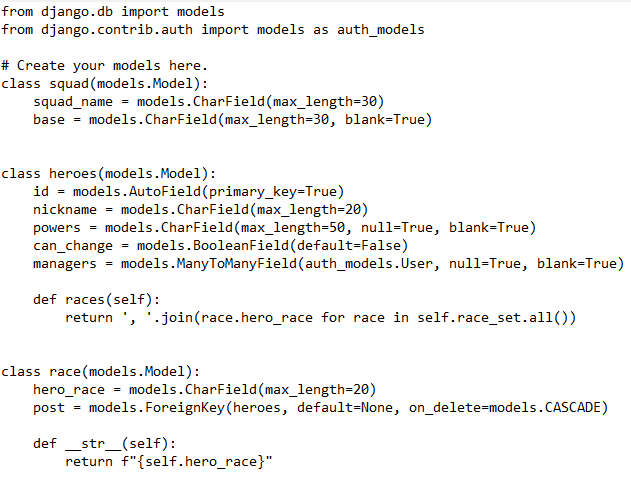
\includegraphics[width=300pt]{./pictures/2-model-example.png}
    \caption[Model příklad]{Ukázka models.py \cite{}}
	\label{fig:Ukázka models.py}                                
\end{figure}

\newpage

\subsection{Django - přídavné balíčky}

Packages, neboli balíčky jsou nástroje pro usnadnění práce s
djangem. Tyto balíčky mají mnoho funkcí, a to od změny vzhledu
stránky, až po implementaci nových funkcí do administrátorské aplikace. Většina
balíčků je tvořena komunitou a každý uživatel si také může vytvořit
svůj vlastní. Pro nalezení vhodného balíčku slouží například stránka
\textit{https://djangopackages.org}, kde lze najít všechna
rozšíření. Ty jsou zpravidla uloženy na stránce \textit{github.com}, kde
je detailně popsána jejich dokumentace. Jejich implementace je opravdu
jednoduchá, pomocí pip se nainstaluje příslušný balíček (např. {\tt pip
install django-rest)}. Dále se v projektu v souboru settings.py přidá
rozšíření do INSTALLED\_APPS a provede se migrace pro
vytvoření tabulek v databázi. \cite{django-packages}

\subsection{Django - administrátorské rozhraní}

Jeden z nejdůležitějších komponentů Djanga je administrátorské
rozhraní, které dovoluje oprávněným uživatelům pracovat s daty
uloženými v databázi. Pomocí registrovaných modelů, může uživatel s
oprávněním prohlížet, přidávat, upravovat a mazat data v jednotlivých
modelech. Administrátorská aplikace je od té uživatelské oddělena a je
možné se do ní dostat přidáním \textit{/admin} za webovou adresu. Pro
přihlášení musí být uživatel registrován jako \textit{staff} a poté mu
musí být udělenu práva k jednotlivým modelům. V aplikaci je možné
nastavit práva jednotlivcům, popřípadě skupinám, do kterých se poté
uživatelé přidávají.

Registrace modelů a jejich následná úprava se prování v souboru
admin.py. Nejprve se modely musí importovat a poté registrovat pro
zobrazení v administrátorském rozhraní. Pokud je potřeba tabulky
modifikovat, například zobrazit jen některá data, je třeba vytvořit ke
každému modelu třídu, která se následně upravuje. Pro tento případ
Django disponuje velkou škálou funkcí pro jednoduchou úpravu zobrazení
dat. \cite{django-admin}

\newpage

\section{Docker}

Docker je open source software používaný pro jednotný vývoj aplikací,
které běží v izolovaných kontejnerech. Je primárně využíván na
operačním systému Linux, ale je možné ho zprovoznit také na Windows
nebo Mac OS X. Výhodou je také, že může běžet jak lokálně, tak na
cloudovém uložišti. Jeho užití spočívá ve vytvoření obrazů (image), ze 
kterých se následně v kontejnerech spustí aplikace ve stejné formě, 
v jaké byl vytvořen její obraz. Díky tomu je poté zajištěn bezproblémový 
chod na jakémkoliv jiném zařízení se stejným operačním systémem. Image 
pro Linux může běžet pouze na systémech s Linux a stejně tak je to pro
Windows. Aplikace spuštěná v Dockeru je izolovaná, a nezasahuje do
ostatních aplikací. Je zde také snadná možnost testovat nové verze
knihoven a aplikací.

Při použití Dockeru je nutné nejprve vytvoří obraz, která obsahuje 
všechny aplikace a jejich nastavení potřebné pro bezproblémový chod. 
Z tohoto obrazu se poté vytvoří kontejner, který obsahuje také svou 
vlastní vrstvu, kde jsou uloženy všechny změny, které uživatel provedl.
\cite{docker}



\section{Git}

Git je open source verzovací systém, který se hojně používá při vývoji
aplikací. Jeho použití je možné na řadě platforem a ovládání
se provádí přes příkazový řádek nebo GUI. Git funguje na principu
repozitářů, ve kterých jsou uloženy projekty. Repozitář obsahuje celý
projekt a jeho kompletní historii provedených změn. Každý člen týmu je
tedy rovněž i zálohou. Při použití Gitu se využívají webové služby
jako například GitHub nebo GitLab, kde jsou repozitáře
zálohovány. Zároveň tu je mnoho užitečných nastavení jako veřejné nebo
soukromé repozitáře, nastavení práv uživatelů a spousta dalších. \cite{git}

\newpage

\section{MariaDB}

MariaDB je komunitně vyvíjeným databázovým systémem odvozeným od MySQL
licencovaný jako svobodný software GNU. První verze MariaDB vyšla v
roce 2009 a měla číslo 5.1, to odpovídalo aktuální verzi MySQL,
poslední verze této řady byla verze 5.5. Další řada nesla označení 10
a lišila se tím, že už nebyla 100\% kompatibilní s MySQL. Aktuálně
nejnovější verze je 10.5, která vyšla na konci roku 2019. MariaDB
podporuje řadu operačních systémů včetně těch nejrozšířenějších jako
Windows, Linux a MacOS. Vzhledem k tomu, že se vycházelo z MySQL, má
MariaDB stejnou strukturu a indexování. Oproti MySQL má ovšem daleko
rychlejší vývoj, což je způsobeno i tím, že je celý projekt open
source. \cite{mariadb}

\section{phpMyAdmin}

Je to open source nástroj pro správu MySQL a MariaDB databáze pomocí
webového rozhraní. Je napsaný v jazyce PHP a je k dispozici ve více jak 70
jazycích včetně češtiny. Toto rozhraní umožňuje provádět SQL příkazy
jako jsou CREATE, DROP, ALTER table a spravovat obsah tabulek. Dále je
zde možno například import dat z CSV souborů, export dat do
nejrůznějších formátů nebo správa uživatelů. K přístupu do rozhraní
phpMyAdmin je zapotřebí webový prohlížeč s podporou cookies a
JavaScriptu. \cite{phpmyadmin} \cite{phpmyadmin-2}

\section{Objektově relační mapování}

Objektově relační mapování (ORM) zajišťuje konverzi dat mezi relační databází a objektově orientovaným programovacím jazykem. Umožňuje konverzi SQL tabulek do tříd a usnadňuje tak práci s psaním SQL dotazů. Pro tuto konverzi se často používají externí programy, které umožňují tyto konverze mezi řadou databázových systémů. Jedním z nich je například SQLAlchemy, které umožňuje tuto konverzi pro programovací jazyk Python a relační databáze SQLite, Postresql, MySQL a další. Některé aplikace včetně Django si ovšem tuto konverzi zprostředkovávají sami za pomoci vlastního ORM. \cite{orm} \cite{sqlalchemy}

\textbf{}
\textit{}




